\begin{landscape}



\begin{figure}[h!]
	\color{blue}
	\centering
	\vspace{-1.2cm}
	\begin{tabular}{c c c}	
		\centering    
		\subfigure[Dataset \code{D1}]{\label{fig:NumOfLibsD1}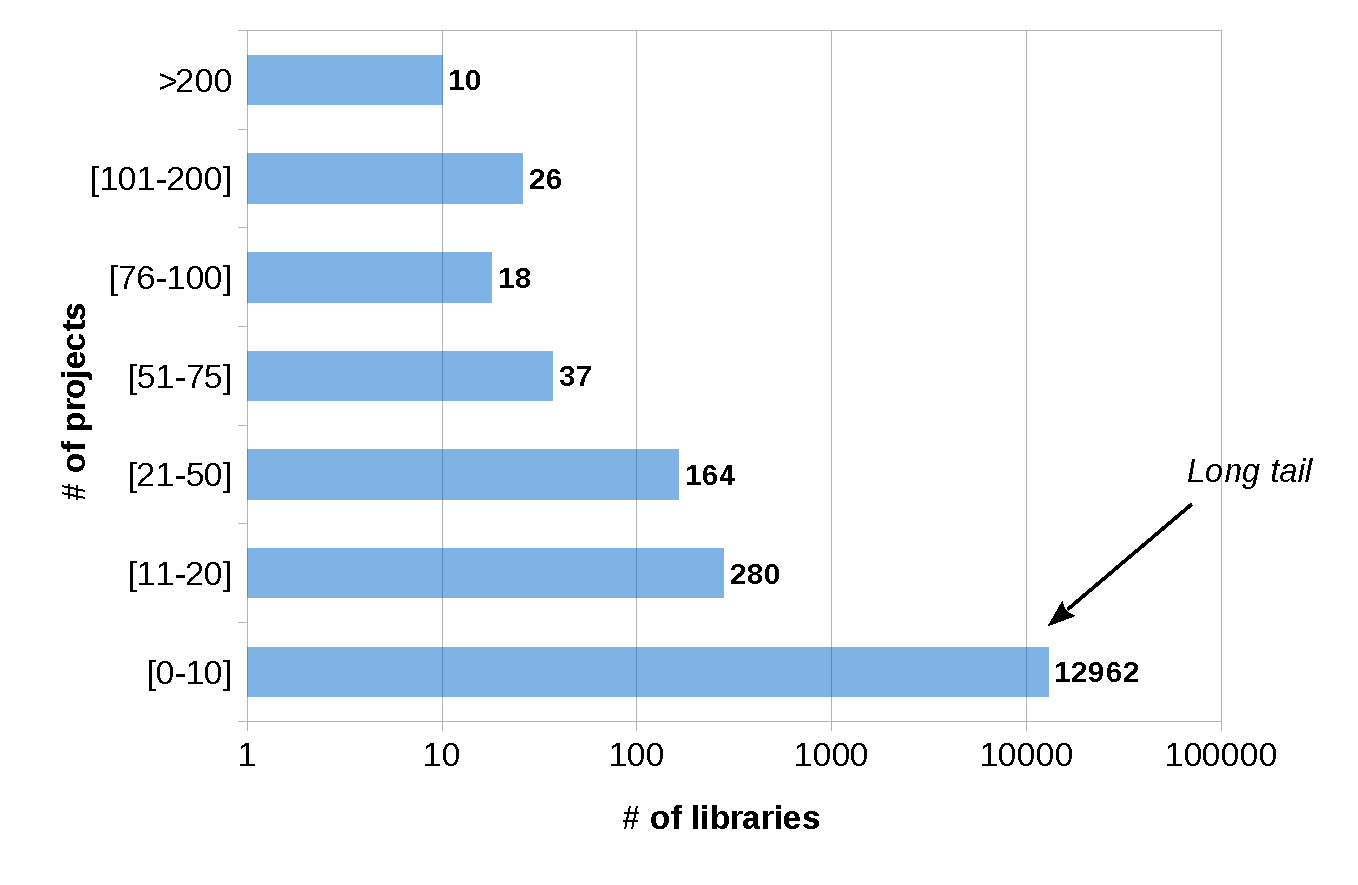
\includegraphics[width=0.50\textwidth]{figs/NumOfLibsCrossRec.pdf}} & 	
		\subfigure[Dataset \code{D2}]{\label{fig:NumOfLibsD2}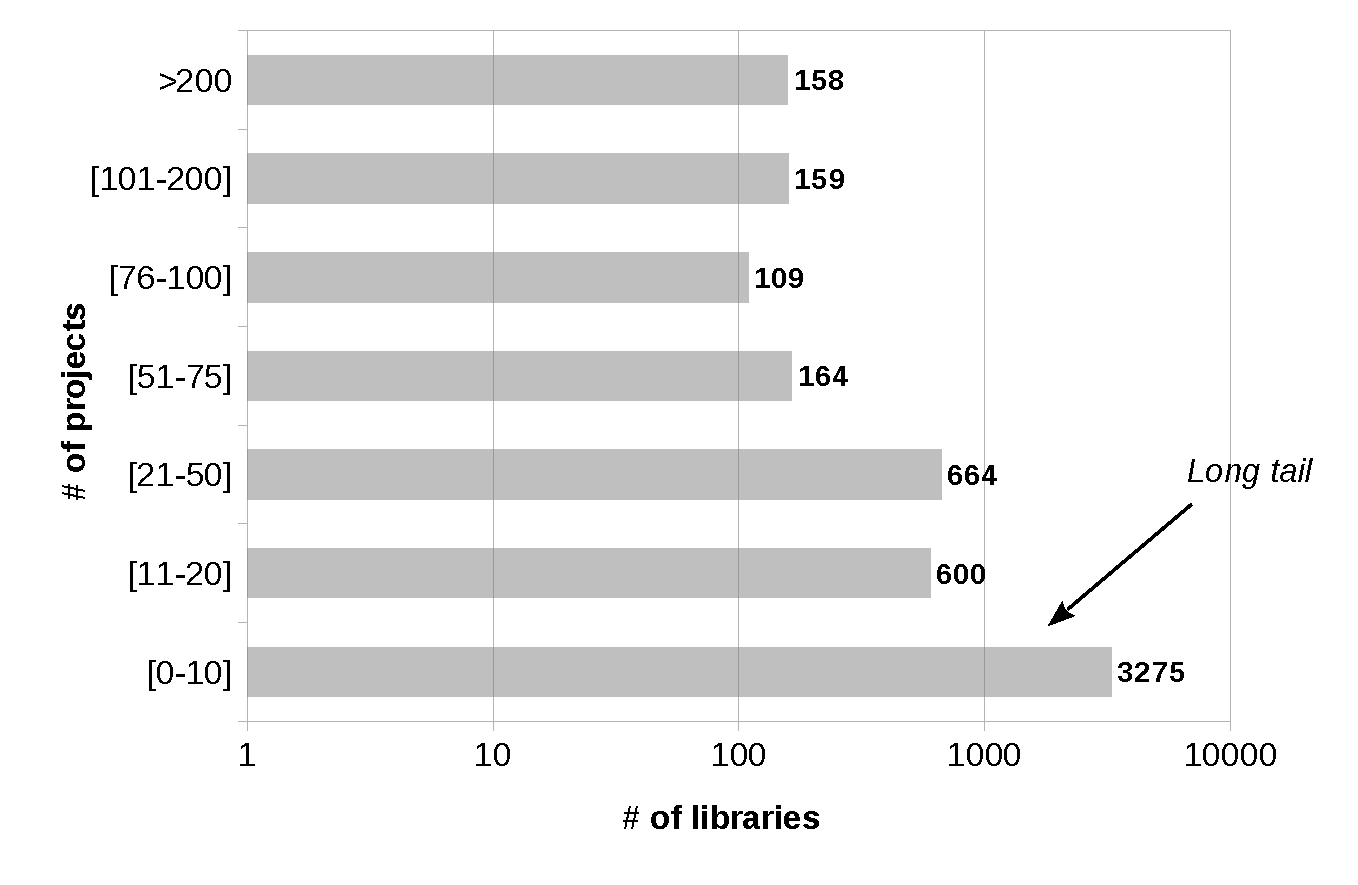
\includegraphics[width=0.50\textwidth]{figs/NumOfLibsLibFinder.pdf}} &
		\subfigure[Dataset \code{D3}]{\label{fig:NumOfLibsD3}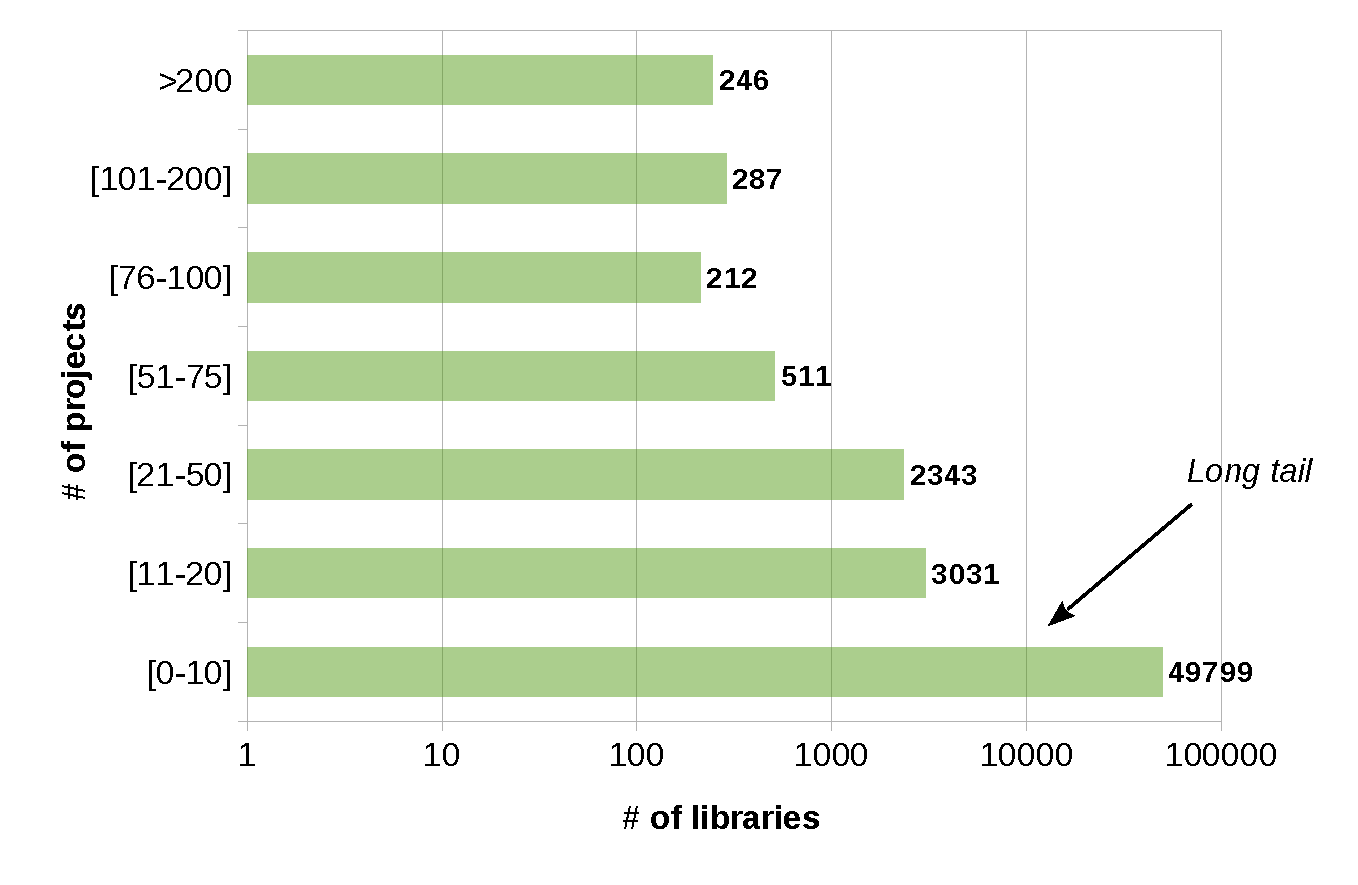
\includegraphics[width=0.50\textwidth]{figs/NumOfLibsLibCUP.pdf}} 
	\end{tabular}
	\label{fig:StatisticsAll}
	\caption{The distribution of libraries.}
\end{figure}

%\vspace{-.5cm}

\begin{figure}[h!]
%	\color{blue}
	\centering
%	\vspace{-1.0cm}
	\begin{tabular}{c c}	
		\centering    
		\subfigure[The projects and their number of forks, commits and pull requests]{\label{fig:ForkCommitPull}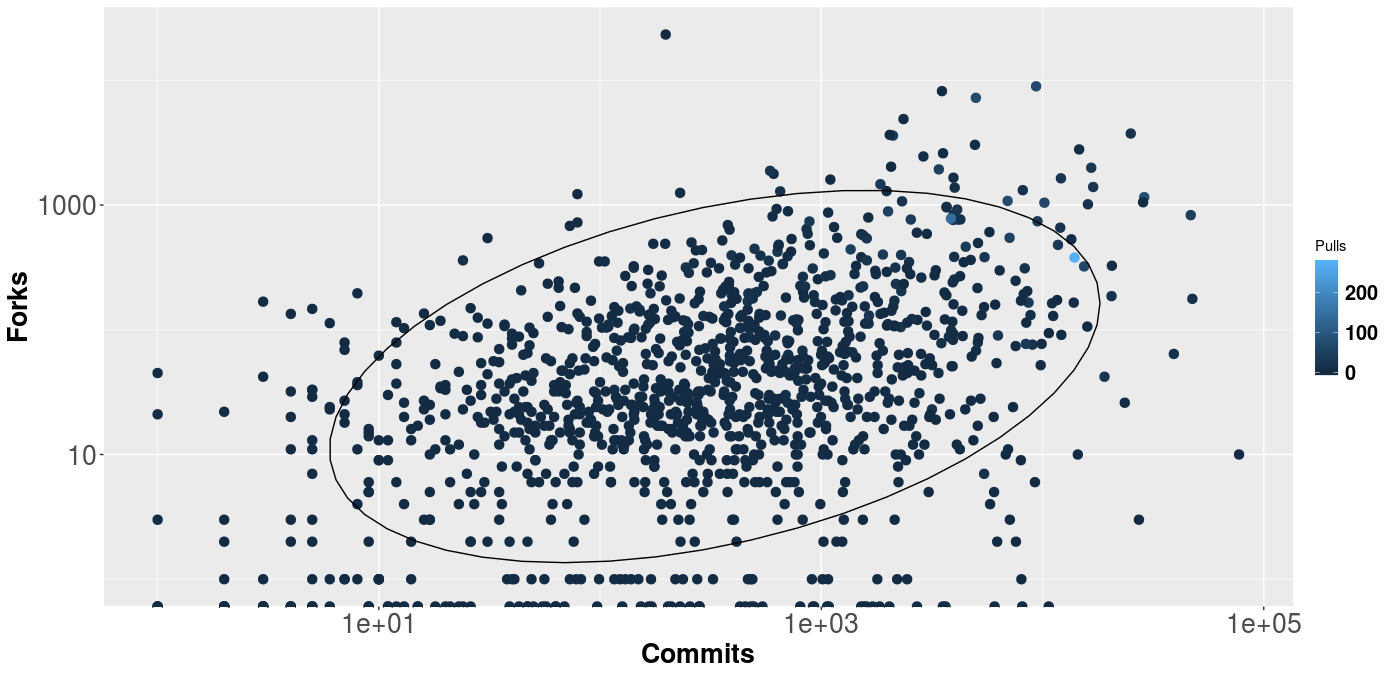
\includegraphics[width=0.80\textwidth]{figs/ForkCommitPull.png}} & 	
		\subfigure[The projects and their number of forks, stars and issues]{\label{fig:ForkStarIssue}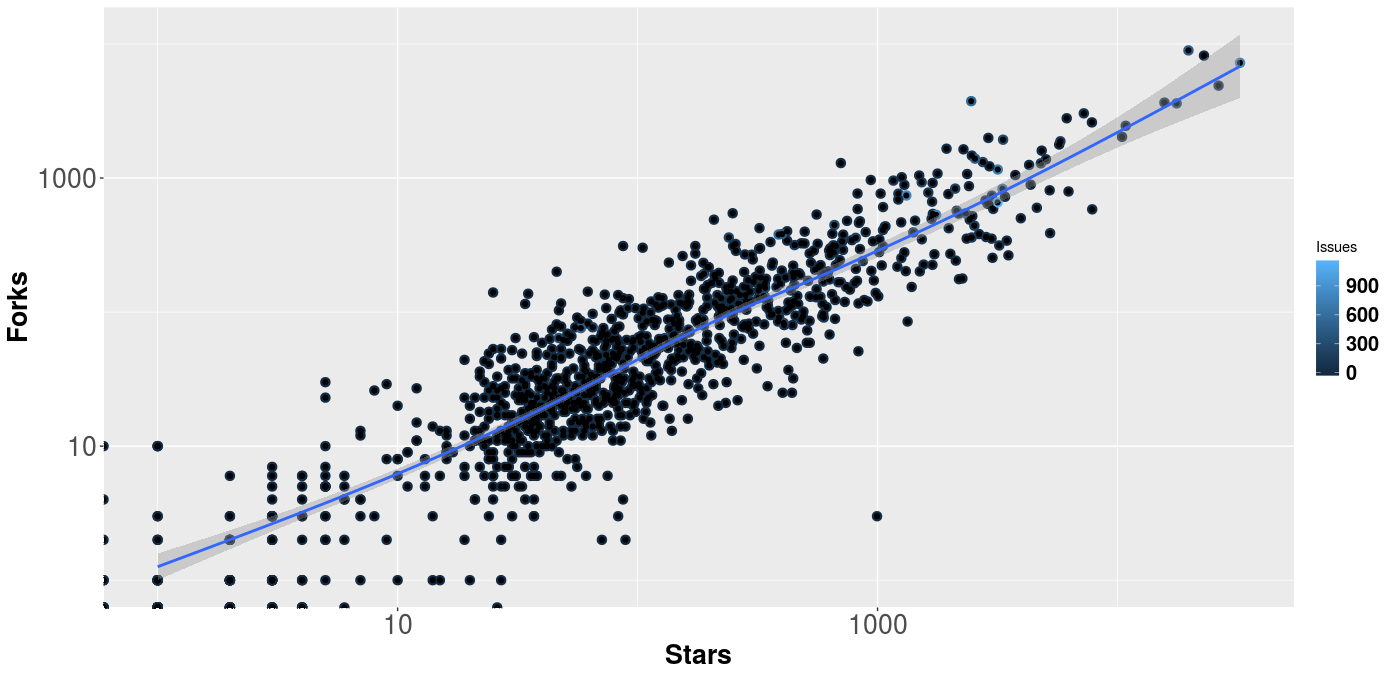
\includegraphics[width=0.80\textwidth]{figs/ForkStarIssue.png}} 
	\end{tabular}
	\label{fig:StatisticsD1}
	\caption{Statistics for Dataset \code{D1}.}
%	\color{black}
\end{figure}



\end{landscape}